

\chapter{A Tour of Computer Systems}


\begin{figure}[h!]
    \centering
    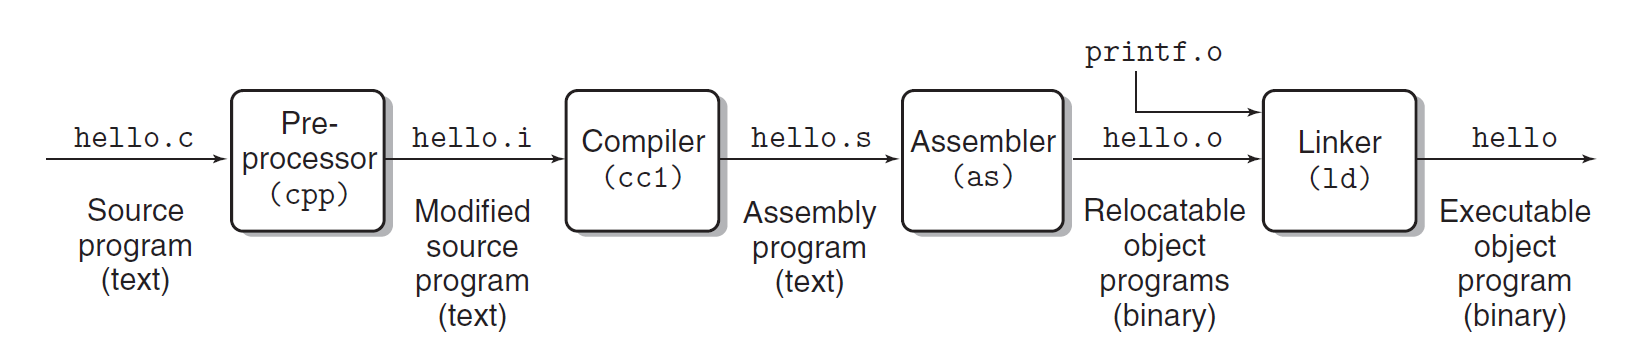
\includegraphics[scale=0.3]{pic/section12/pic1}
    \caption{The compilation system.}
\end{figure}

linux> gcc -o hello hello.c

컴파일 시스템을 이해해야하는 이유

\begin{enumerate}
    \item 성능 최적화
    \item 링커 에러 이해하기
    \item 보안 약점
\end{enumerate}


\begin{figure}[h!]
    \centering
    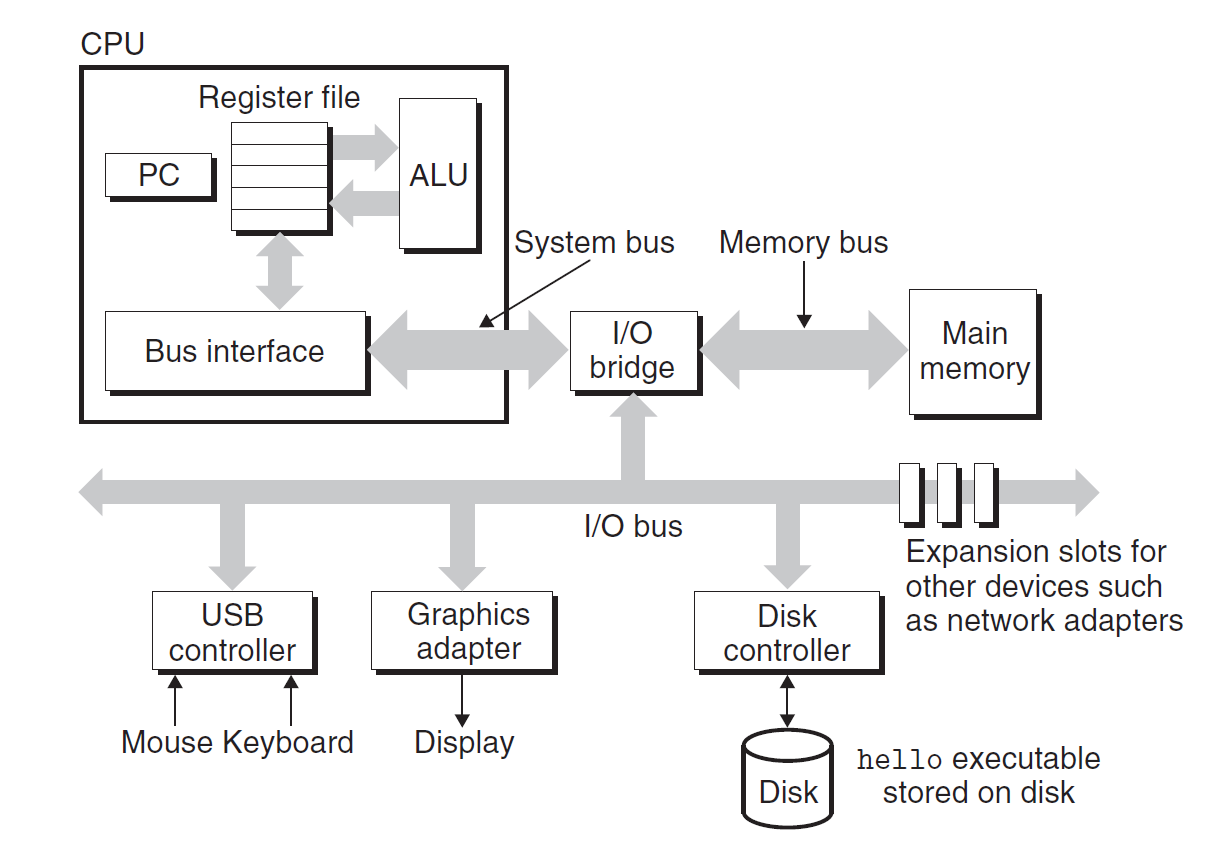
\includegraphics[scale=0.5]{pic/section12/pic2}
    \caption{Hardware organization
    of a typical system. CPU:
    central processing unit,
    ALU: arithmetic/logic unit,
    PC: program counter, USB:
    Universal Serial Bus.}
\end{figure}


\begin{itemize}
    \item Buses
    
    하드웨어에 돌아다니는 데이터 통로(a collection of electrical conduits) word라고 하는 고정크기의 바이트 단위로 데이터가 전송된다. 최근에는 4byte 또는 8byte 크기를 가진다.

    \item I/O Devices
    시스템과 외부로부터의 연결을 가능케하는 장치.

    \item Main Memory
    
    프로세서가 프로그램을 실행하는 동안 데이터와 프로그램을 저장하는 임시 저장장치이다. 물리적으로 DRAM(Dynamic Random Access Memorry)로 구성되어 있다.

    \item Processor(CPU)
    
    프로그램 카운터(PC)는 메인메모리의 기계어 인스트럭션을 가리키는데 이 인스트럭션 값을 읽어서 특정한 동작을 수행하고 PC값을 갱신한다. 이 동작은 메인 메모리, 레지스터 파일, ALU주위를 돈다.
    레지스터 파일은 고유의 이름을 갖는 워드 크기의 레지스터 집합이다.
\end{itemize}

추가적인것 .

캐시

메모리 계층

쓰레드 동시성

프로세스 contex switching

가상메모리

파일

네트워크


\begin{figure}[h!]
    \centering
    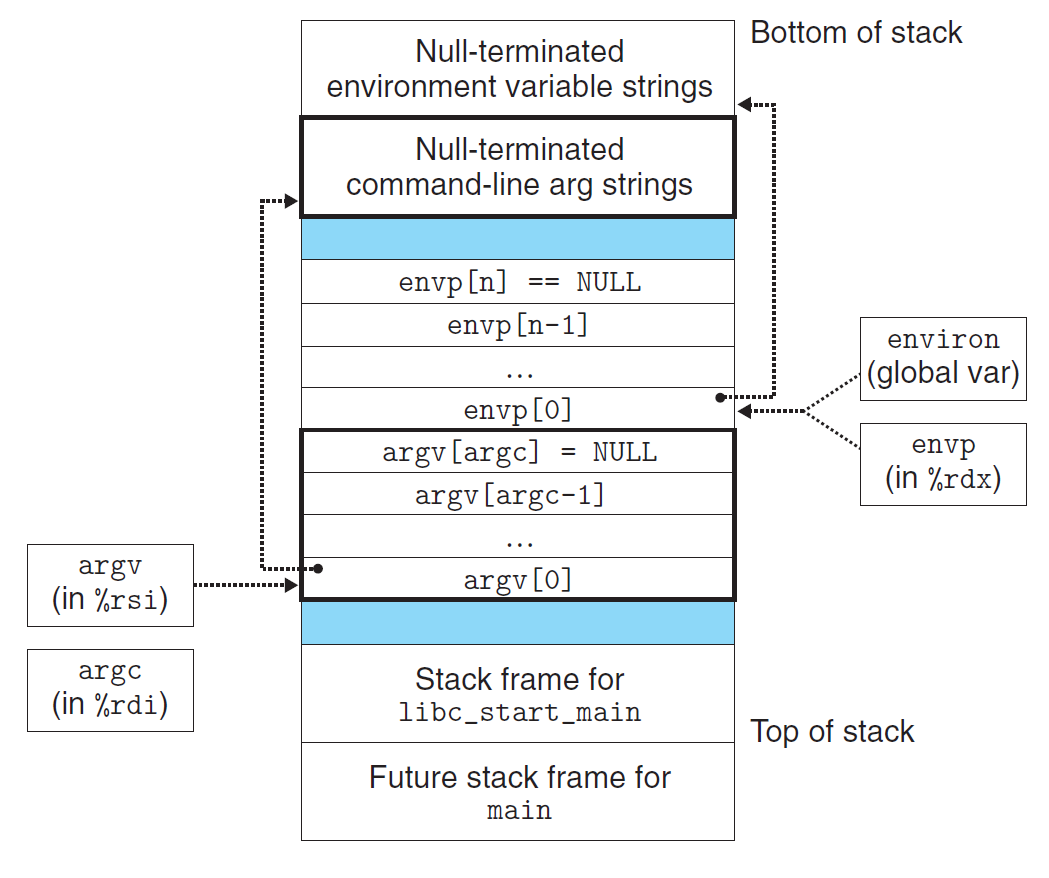
\includegraphics[scale=0.5]{pic/section12/pic3.png}
    \caption{메모리 계층}
\end{figure}



\begin{figure}[h!]
    \centering
    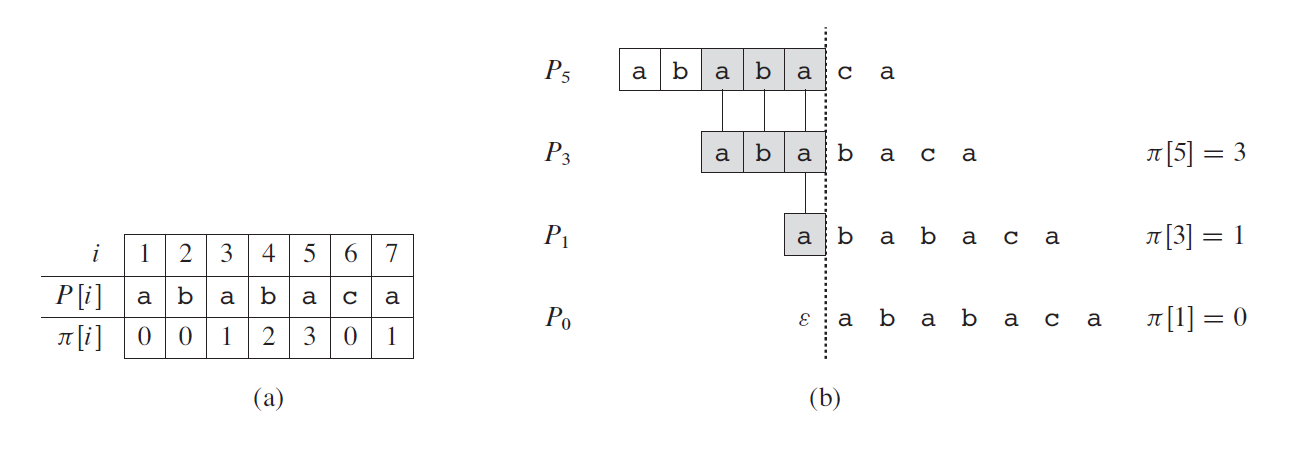
\includegraphics[scale=0.5]{pic/section12/pic4.png}
    \caption{Layered view of a computer system.}
\end{figure}



\begin{figure}[h!]
    \centering
    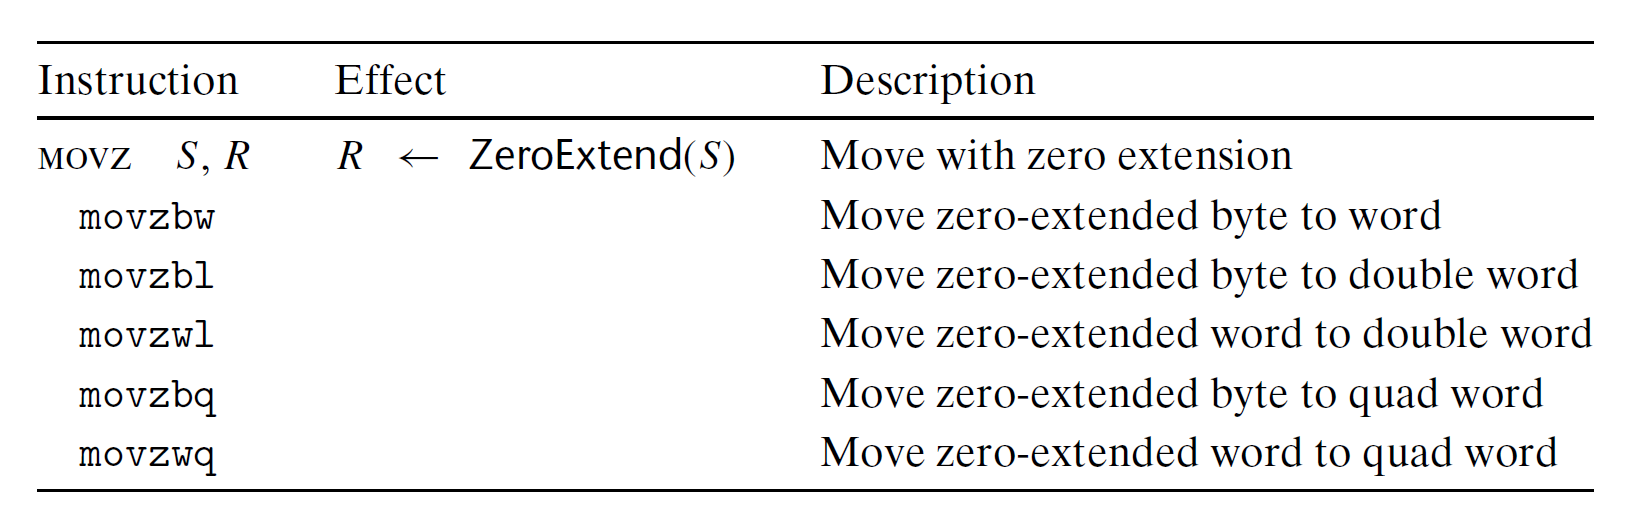
\includegraphics[scale=0.5]{pic/section12/pic5.png}
    \caption{Abstractions provided by an operating system.}
\end{figure}


\begin{figure}[h!]
    \centering
    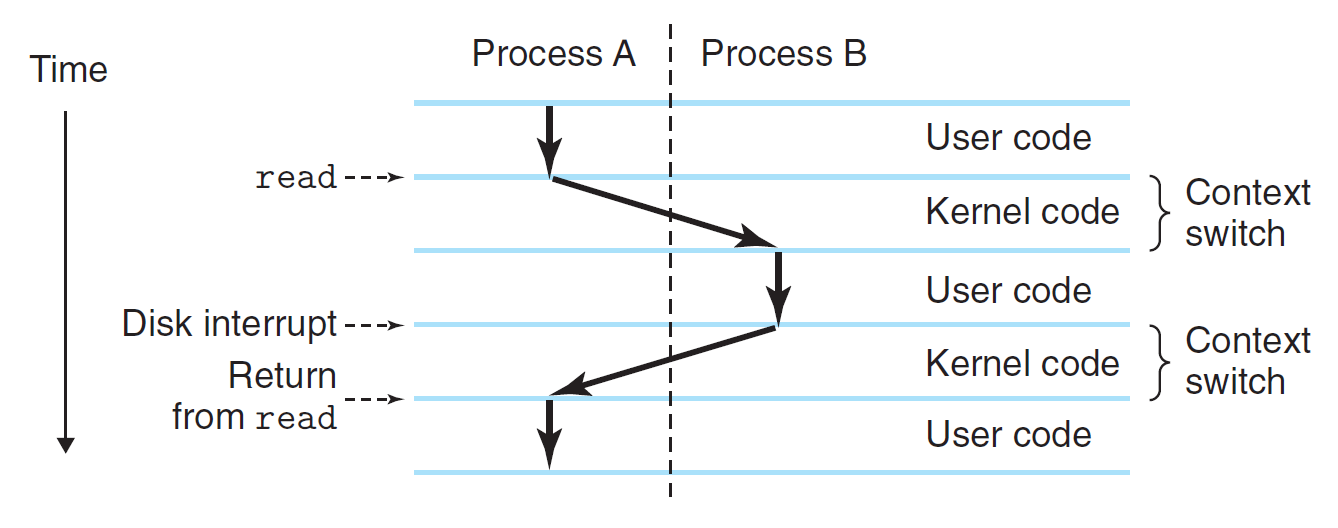
\includegraphics[scale=0.4]{pic/section12/pic6.png}
    \caption{context switching}
\end{figure}

\begin{figure}[h!]
    \centering
    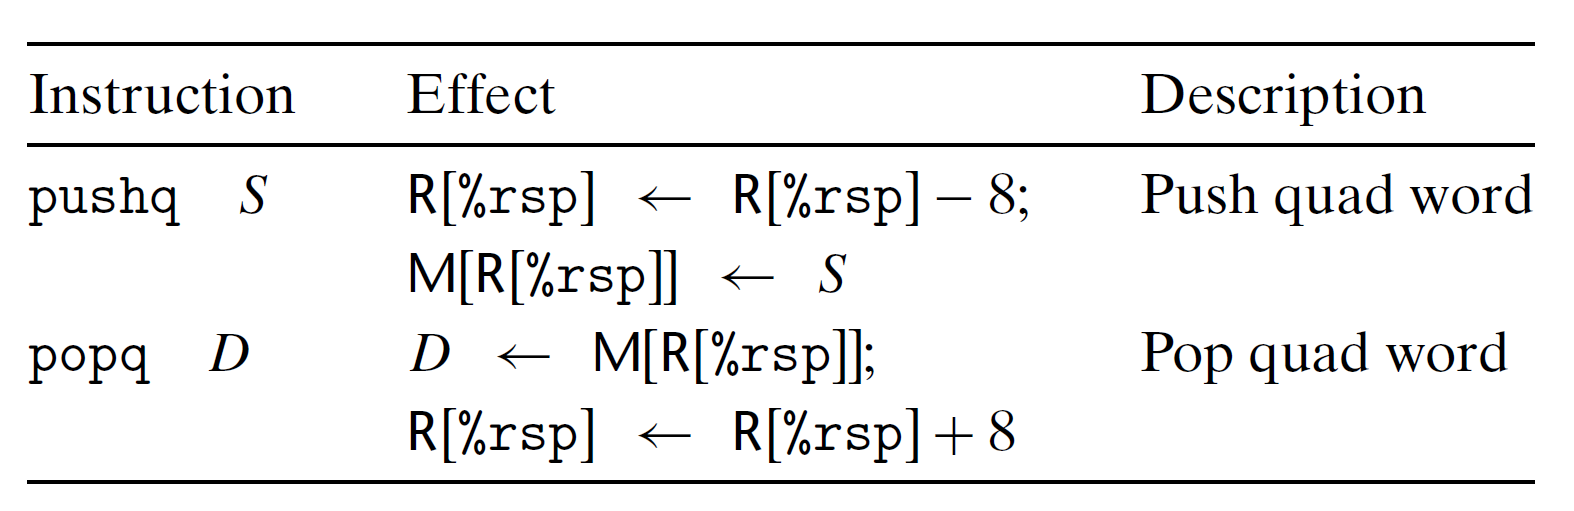
\includegraphics[scale=0.5]{pic/section12/pic7.png}
    \caption{Process virtual address space.}
\end{figure}

\begin{figure}[h!]
    \centering
    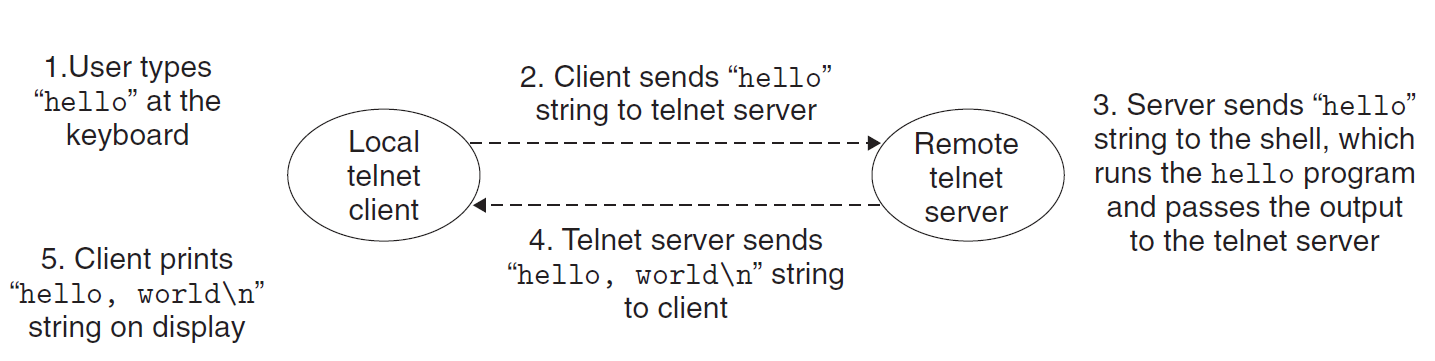
\includegraphics[scale=0.4]{pic/section12/pic8.png}
    \caption{Using telnet to run hello remotely over a network.}
\end{figure}

\begin{figure}[h!]
    \centering
    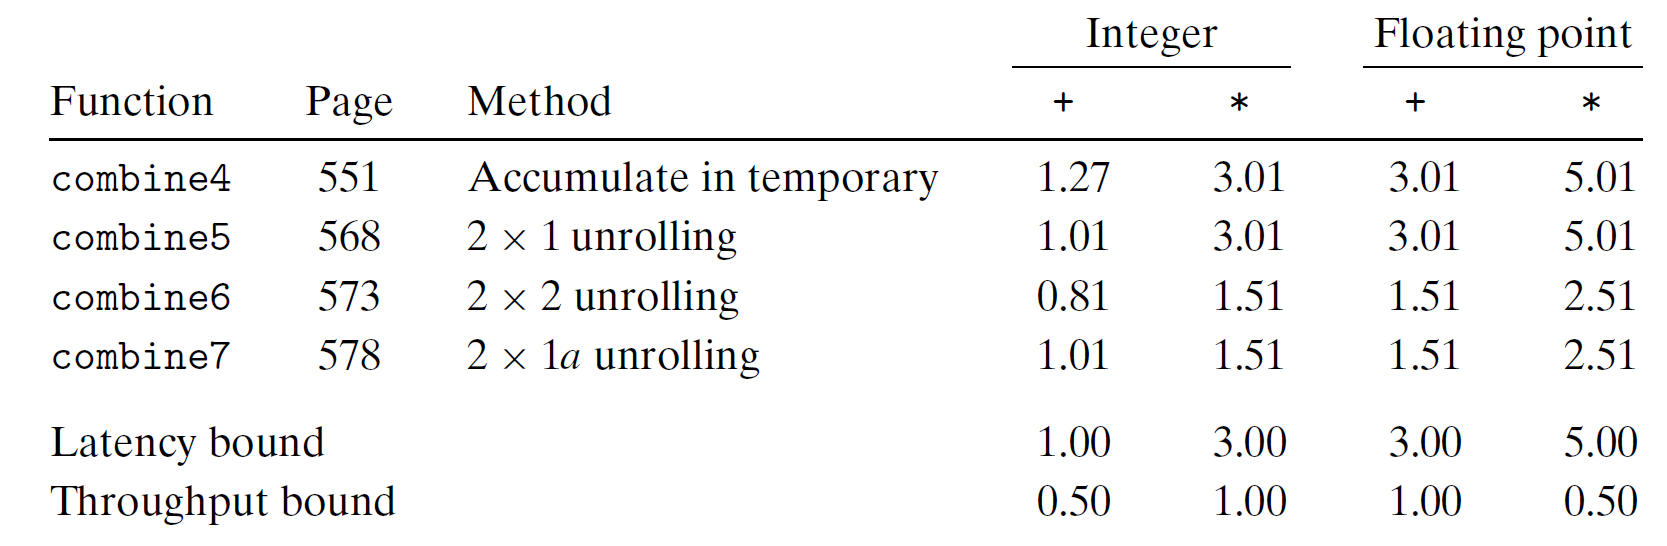
\includegraphics[scale=0.5]{pic/section12/pic9.png}
    \caption{Multi-core processor organization. Four processor cores are integrated onto a single chip.}
\end{figure}


\begin{figure}[h!]
    \centering
    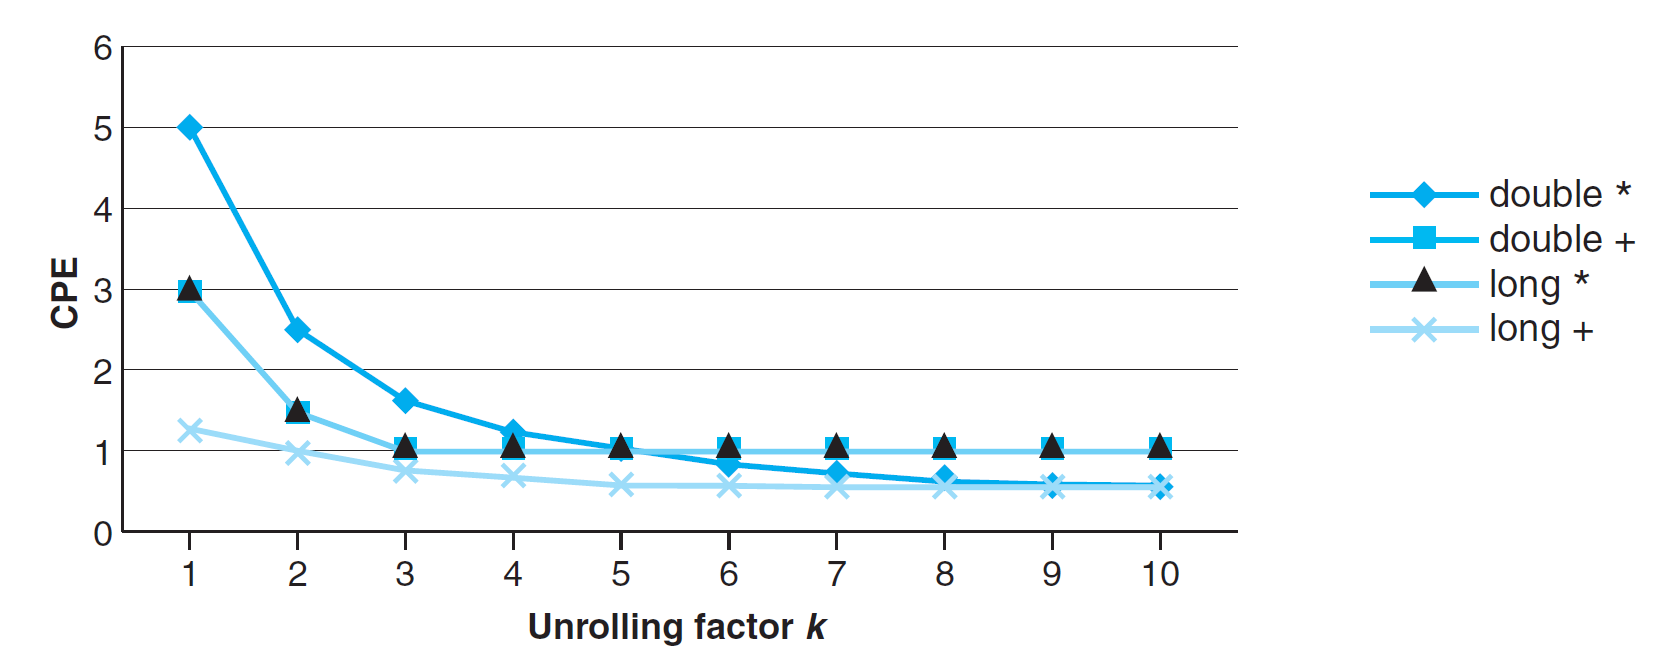
\includegraphics[scale=0.3]{pic/section12/pic10.png}
    \caption{Some abstractions provided by a computer system}
\end{figure}


%\chapter{Part I Program Structure and Execution}
\part{Part I Program Structure and Execution}

\chapter{Representing and Manipulating Information}


메모리에 객체가 저장되는 방식

객체의 수조는 사용된 바이트의 최소 주소로 정함.
4byte크기인 int type 변수 x가 주소 0x100로 설정된다면 $int \&x$의 값은 0x100이고 주소 0x100,1,2,0x103에 x가 저장된다.






\begin{figure}[h!]
    \centering
    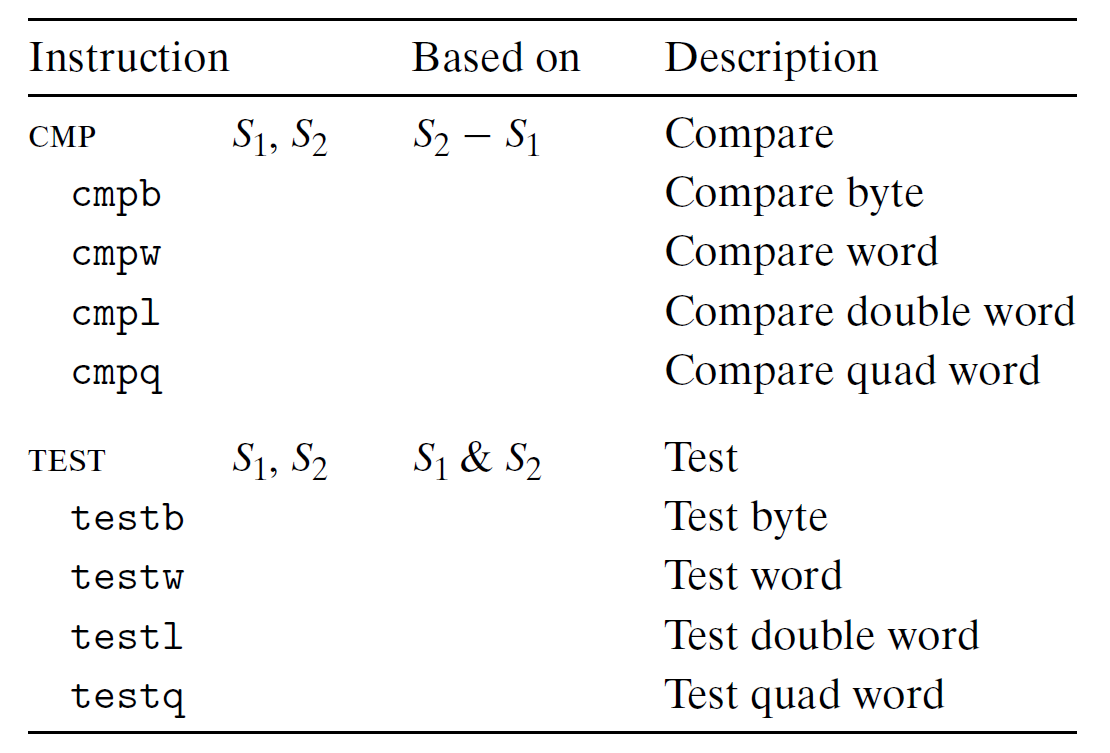
\includegraphics[scale=0.3]{pic/section12/pic11.png}
    \caption{ex endian}
\end{figure}


\begin{itemize}
    \item little endian :  최하위 바이트를 시작주소에 차례로 저장하는 방식 (intel)
    \item big endian : 최상위 바이트를 시작주소에 차례로 저장하는 방식 (IBM Oracle)
\end{itemize}


\begin{lstlisting}[style = CStyle]
 #include <stdio.h>
 typedef unsigned char *byte_pointer;

 void show_bytes(byte_pointer start, size_t len) {
 int i;
 for (i = 0; i < len; i++)
 printf(" %.2x", start[i]);
 printf("\n");
 }

 void show_int(int x) {
 show_bytes((byte_pointer) &x, sizeof(int));
 }

 void show_float(float x) {
 show_bytes((byte_pointer) &x, sizeof(float));
 }

 void show_pointer(void *x) {
 show_bytes((byte_pointer) &x, sizeof(void *));
 }


 void test_show_bytes(int val) {
     int ival = val;
     float fval = (float) ival;
     int *pval = &ival;
     show_int(ival);
     show_float(fval);
     show_pointer(pval);
     }

\end{lstlisting}
서로 다른 컴퓨터 타입은 서로 다르고, 호환성이 없는 인스트럭션과 인코딩을 사용한다. 다른 운영체제를 실행하는 동일한 프로세서들도 각자의 코딩 관습에 차이가 잇으며, 따라서 이들은 바이너리 호환성을 갖지 못한다.

\begin{lstlisting}[style = CStyle]
    void inplace_swap(int *x, int *y) {
     *y = *x ^ *y; /* Step 1 */
     *x = *x ^ *y; /* Step 2 */
     *y = *x ^ *y; /* Step 3 */
     }
    \end{lstlisting}
    
    
    Shift Operations in C
    
    \begin{itemize}
        \item  논리(logical) 우측 쉬프트 : 좌측 끝을 k개의 0으로 채운다.
        \item  산출(arithmetic) 우측 쉬프트 : 좌측 끝을 k개의 1로 채운다.
    \end{itemize}
    
    \begin{figure}[h!]
        \centering
        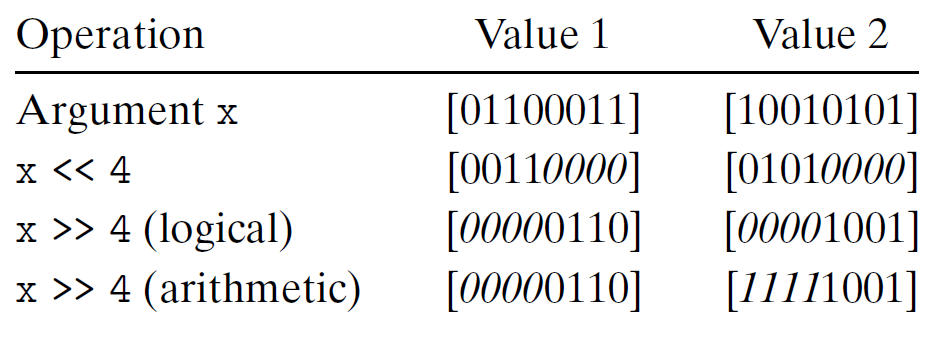
\includegraphics[scale=0.4]{pic/section12/shift}
    \end{figure}
    
